\documentclass[t]{beamer}

\usepackage[english]{babel}
\usepackage{graphicx}
\usepackage{subcaption}
\usepackage{tabularx}
\usepackage{algorithm}
\usepackage{algpseudocode}
\usepackage{tikz}
\usepackage{gensymb}
\usepackage{pgfplots}
\usepackage{xcolor}
\usepackage{hyperref}



\definecolor{lightblue}{rgb}{0.68, 0.85, 0.9}
\definecolor{darkblue}{rgb}{0.2, 0.2, 0.6}
\definecolor{lightred}{rgb}{1.0, 0.6, 0.6}
\definecolor{darkred}{rgb}{0.7, 0.1, 0.1}
\definecolor{warmorange}{rgb}{1.0, 0.5, 0.0}
\definecolor{forestgreen}{rgb}{0.0, 0.6, 0.3}
\definecolor{plumpurple}{rgb}{0.5, 0.2, 0.5}


\graphicspath{{./images/}}


\usetikzlibrary{arrows.meta}
\usetikzlibrary{automata}
\tikzset{
  every state/.style={
    draw,
    minimum size=0.3cm, 
    inner sep=0.5pt,  
    align=center,
    font=\footnotesize
  }
}
\tikzset{>={Latex[width=1.5mm,length=2.5mm]}}
\tikzset{every picture/.style=thick}


\usetheme{Copenhagen}
\setbeamertemplate{footline}{}
\setbeamertemplate{headline}{}
\setbeamertemplate{navigation symbols}{}
\addtobeamertemplate{navigation symbols}{}{%
    \usebeamerfont{footline}%
    \setbeamercolor{footline}{fg=blue}
    \usebeamercolor[fg]{footline}%
    \hspace{3em}%
    \begin{small}
        \insertframenumber
    \end{small}   
}


\title{\Large Partially Optimal Cubic Subspace Clustering}
\subtitle{\small Research Project Machine Learning}
\author{Volodymyr Drobitko}
\institute{Technische Universität Dresden}
\date{21.07.2025}


% sets
\newcommand{\nat}{\mathbb{N}} % natural numbers
\newcommand{\real}{\mathbb{R}} % real numbers
\newcommand{\fSet}{S} % finite set of samples
\newcommand{\bSet}{\{0,1\}} % boolean set
\newcommand{\subR}{R} % sample subset

% constants
\newcommand{\noise}{\sigma} % noise for the plane points
\newcommand{\maxD}{D} % max distance for the plane points
\newcommand{\tol}{10^{-6}} % tolerance

% functions
\DeclareMathOperator{\cost}{c} % cost function
\DeclareMathOperator{\labels}{y} % label function

% \includeonly{experiments}

\begin{document}

\frame{\titlepage}
%%% contents
\section{Introduction}
\frame{\tableofcontents[currentsection]}


\begin{frame}
    \frametitle{Problem Statement (1)}
    \onslide<1->{
        Finite sample set $\fSet$, 
        cost function $\cost \colon \binom{\fSet}{3} \to \real$.\\
        Instance of the \textbf{Cubic Clique Partition Problem}:\\
        \[
        \max\limits_{\labels \colon \binom{\fSet}{2} \to \bSet}
        \sum\limits_{\{a,b,c\} \in \binom{\fSet}{3}}
        \cost_{\{a,b,c\}}\labels_{\{a,b\}}\labels_{\{b,c\}}\labels_{\{a,c\}} 
        \]
        subject to 
        $\labels_{\{a,b\}} + \labels_{\{b,c\}} - 1 \leq \labels_{\{a,c\}}$
        for all distinct $a,b,c \in \fSet$.    
    }
    \vspace{25px}
    \onslide<2->{
        Find a \textbf{partially optimal solution}, i.e.
        fix some labels $\labels_{\{a,b\}}$
        for distinct $a,b \in \fSet$
        \[
        \begin{cases}
            \labels_{\{a,b\}}=1 & \text{join } a,b\\
            \labels_{\{a,b\}}=0 & \text{cut } a,b\\
            \labels_{\{a,b\}}=\text{?} & \text{unknown}
        \end{cases}
        \]
        in such way that there still exists
        an optimal solution. 
    }
\end{frame}

\begin{frame}
    \frametitle{Problem Statement (2)}
    \textbf{Subspace Instances} of the Cubic Clique Partition Problem
    \vspace{5px}
    \onslide<1->{
        Samples $\fSet$: points $\fSet \subset \real^3$\\
    }
    \onslide<2->{
        Point generation: 3 distinct planes containing the origin, noise $\noise$\\
    }
    \onslide<3->{
        Optimal clustering $\labels^*$: original planes\\
    }
    \onslide<4->{
        Cost function $\cost$? (no concrete plane info given)
    }
    \begin{figure}[h]
    \centering
        \onslide<1->{
            \begin{subfigure}{0.4\textwidth}
                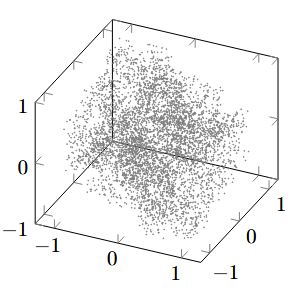
\includegraphics[width=\textwidth]{gray-points}
                \caption{Samples $\fSet$}
            \end{subfigure}
        }
        \hfill
        \onslide<2->{
            \begin{subfigure}[b]{0.4\textwidth}
                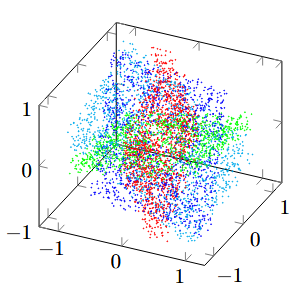
\includegraphics[width=\textwidth]{colored-points}
                \caption{Optimal clustering $\labels^*$}
            \end{subfigure}
        }
        \hspace{0.1\textwidth}
    \end{figure}
\end{frame}


\begin{frame}
    \frametitle{Research Goals and Contributions}
    \begin{tabularx}{\textwidth}{p{0.5\textwidth}|X}
        \textbf{Task} & \textbf{Solution}\\
        \hline 
        \onslide<1->{
        \vspace{-7px}
        read
        `Partial Optimality in Cubic Correlation Clustering'
        \cite{TODO};
        implement the algorithm for establishing partial optimality
        to the cubic clique partition problem;
        } &
        \onslide<2->{
        \vspace{-7px}
        my own implementation in C++ of the suggested
        algorithm with some adjustments
        \\
        \hline
        }
        \onslide<3->{
        \vspace{-7px}
        construct subspace instances
        of increasing difficulty
        by generating the sample points
        and by defining a
        \textbf{suitable cost function}
        for the point triples
        } &
        \onslide<4->{
        \vspace{-7px}
        point generation using the linear algebra methods;
        experimentally determined geometric
        cost function 
        with a significant noise tolerance;
        \\
        \hline
        }
        \onslide<5->{
        \vspace{-7px}
        apply the algorithm to the constructed subspace instances,
        assess partial optimality, accuracy with respect to
        truth, and computation time
        } &
        \onslide<6->{
        \vspace{-7px}
        systematic empirical assessment
        of the algorithm application the the problem subspace instances 
        with my cost function proving its quality
        }
    \end{tabularx}
\end{frame}
\section{Partial Optimality for Cubic Clique Partition Problem}
\frame{\tableofcontents[currentsection]}


\begin{frame}
    \frametitle{Partial Optimality for Cubic Clique Partition Problem}
    % mention triple, pairs and constant!!!
    % fix labels if something holds
    % improving map
    % reformulate the problem
    % 2 correct join conditions cannot be combined in the optimal solution
    % so when applied simultaneously they result into a suboptimal solution. 
    \onslide<1->{
        Extended cost function
        $\cost \colon \binom{\fSet}{3} \cup \binom{\fSet}{2} \cup {\emptyset} \to \real$\\
    }
    \vspace{5px}
    \onslide<2->{
        Instance of the extended cubic clique partition problem:
        \[
            \min\limits_{\labels \colon \binom{\fSet}{2} \to \bSet}
            \sum\limits_{\{a,b,c\} \in \binom{\fSet}{3}}
            \cost_{\{a,b,c\}}\labels_{\{a,b\}}\labels_{\{b,c\}}\labels_{\{a,c\}} 
            + \cost_{\{a,b\}}\labels_{\{a,b\}}
            + \cost_{\emptyset}
        \]\\
    }
    \vspace{5px}
    \onslide<3->{
        Construct \textbf{Improving Maps} for the clustering $\labels$\\
    }
    \vspace{5px}
    \onslide<4->{ 
    $\to$ \textbf{Partial Optimality Conditions:}
    \vspace{5px}
    \begin{enumerate}
        \onslide<5->{
        \item Subproblem-CUT-condition (cut subset from its complement)
        }
        \onslide<6->{
        \item CUT-conditions (cut pairs and triples)
        }
        \onslide<7->{
        \item JOIN-conditions (join subsets, pairs and triples)\\
        }
    \end{enumerate}
    }
    \vspace{5px}
    \onslide<8->{
    CUT-conditions can be applied simultaneously\\
    JOIN-conditions cannot be applied simultaneously!\\
    }
    \vspace{5px}
    \onslide<9->{
    Apply partial optimality connditions $\to$ solve subproblems\\    
    }
\end{frame}

\begin{frame}
    \frametitle{Partial Optimality Algorithm}
    \onslide<1->{
    \textbf{Partial Optimality Algorithm:\\}
    \hspace{10px}\textbf{Input:} clustering $\labels$ without fixed labels
    \begin{algorithmic}
        \While{condition applied}
            \State apply subproblem-CUT-condition exhaustively
            \State apply one of JOIN-conditions (in effective order)
        \EndWhile
        \State apply CUT-conditions exhaustively
    \end{algorithmic}
    \hspace{10px}\textbf{Output:} partially optimal clustering $\labels$ with some fixed labels
    }
    \vspace{10px}
    \onslide<2->{
    \textbf{Reduction to subproblems:}
    \begin{enumerate}
        \item Subproblem-CUT-condition:
        fix CUT labels for element pairs from different sample subsets; 
        solve each subset as an independent problem and accumulate the results in $\cost_{\emptyset}$;
        \onslide<3->{
        \item JOIN-Conditions: 
        fix JOIN labels for elements of the sample subset; 
        add the join-cost to $\cost_{\emptyset}$;
        solve the problem where the subset is considered as one sample;
        }
    \end{enumerate}
    }
\end{frame}

\begin{frame}
    \frametitle{Subproblem-CUT and Subset-JOIN}
    % A couple of words about the split and the implementation
    % apply exhaustively
    % intuition 3.1 and 3.11!!!
    % 3.11 adjustment
    \onslide<1->{
    \textbf{Subproblem-CUT:} cut sample subsets $\subR_1, \subR_2, \dots, \subR_k$
    that are only connected via non-negative costs (applied if $k > 1$)\\
    }
    \vspace{5px}
    \onslide<2->{
    \textbf{Subset-JOIN:} join sample subset $\subR$ with only non-positive costs
    if its worst bipartition joining cost is less than or equal to
    the reward of joining $\subR$ with $\overline{\subR}$ (applied if $|\subR| > 1$)\\
    (The worst bipartition joining cost $\approx$ min-cut)\\
    }
    \vspace{15px}
    \onslide<3->{
        \begin{tikzpicture}[node distance=30px]
            % nodes
            \node[state] (a) {a};
            \node[state] (b) [below left of=a] {b};
            \node[state] (c) [below right of=b] {c};
            \node[state] (d) [above right of=c] {d};
            \node[state] (e) [below right of=d] {e};
            \node[state] (f) [above right of=e] {f};
            \node[state] (h) [below of=e] {h};
            \node[state] (g) [above of=d] {g};
            \node[state] (i) [above of=f] {i};
            % edges
            \path[-] (a) edge node[below right=3px, below] {\footnotesize -1} (b);
            \path[-] (a) edge node {} (c);
            \path[-] (b) edge node {} (c);
            \path[-] (a) edge node[below left=3px, below] {\footnotesize -15} (d);
            \path[-] (c) edge node {} (d);
            \path[-] (d) edge node {} (g);
            \path[-] (d) edge node {} (f);
            \path[-] (g) edge node {} (i);
            \path[-] (i) edge node[above left] {\footnotesize -10} (f);
            \path[-] (g) edge node[below left] {\footnotesize -2} (f);
            \path[-] (d) edge node {} (e);
            \path[-] (e) edge node {} (f);
            \path[-] (e) edge node {} (h);
            \path[-] (d) edge node[right=-3px] {\tiny 50} (h);
            \path[-] (h) edge node[left=-4px] {\tiny -50} (f);
        \end{tikzpicture}
    }
    \hspace{5px}
    \onslide<4->{
        \begin{tikzpicture}[node distance=30px]
            % nodes
            \node[state] (acd) {acd};
            \node[state] (b) [left of=acd] {b};
            \node[state] (e) [below right of=acd] {e};
            \node[state] (f) [above right of=e] {f};
            \node[state] (h) [below of=e] {h};
            \node[state] (g) [above of=acd] {g};
            \node[state] (i) [above of=f] {i};
            % edges
            \path[-] (acd) edge node[above] {\footnotesize -1} (b);
            \path[-] (acd) edge node {} (g);
            \path[-] (acd) edge node {} (f);
            \path[-] (g) edge node {} (i);
            \path[-] (i) edge node[above left] {\footnotesize -10} (f);
            \path[-] (g) edge node[below left] {\footnotesize -2} (f);
            \path[-] (acd) edge node {} (e);
            \path[-] (e) edge node {} (f);
            \path[-] (e) edge node {} (h);
            \path[-] (acd) edge node[right=-3px] {\tiny 50} (h);
            \path[-] (h) edge node[left=-4px] {\tiny -50} (f);
        \end{tikzpicture}
    }
    \onslide<5->{
        \begin{tikzpicture}[node distance=30px]
            % nodes
            \node[state] (acd) {acd};
            \node[state] (b) [above of=acd] {b};
            \node[state] (efghi) [below of=acd] {efghi};
            % edges
            \path[-] (acd) edge node[right] {\footnotesize -1} (b);
            \path[-] (acd) edge node[right] {\footnotesize 48} (efghi);
        \end{tikzpicture}
    }
    \onslide<6->{
        \begin{tikzpicture}[node distance=30px]
            % nodes
            \node[state] (acd) {acd};
            \node[state] (b) [above of=acd] {b};
            \node[state] (efghi) [below of=acd] {efghi};
            % edges
            \path[-] (acd) edge node[right] {\footnotesize -1} (b);
        \end{tikzpicture}
    }
    \onslide<7->{
        \begin{tikzpicture}[node distance=30px]
            % nodes
            \node[state] (abcd) {abcd};
            \node[state] (efghi) [below of=acd] {efghi};
        \end{tikzpicture}
    }
    \\
    \hspace{20px}
    \onslide<3->{$\cost_{\emptyset}=0$}
    \hspace{60px}
    \onslide<4->{$\cost_{\emptyset}=-15$}
    \hspace{25px}
    \onslide<5->{$\cost_{\emptyset}=-75$}
    \hspace{15px}
    \onslide<7->{$\cost_{\emptyset}=-76$}
\end{frame}


\begin{frame}
    \frametitle{Other JOIN-conditions}
    \onslide<1->{
        \textbf{Pair-JOIN-1:} join samples $i,j$ if
        their overall joining reward $\geq$
        the sum of rewards and penalties for joining
        some subset $\subR$ with $i \in \subR$ 
        and $\overline{\subR}$ with $j \in \overline{\subR}$
        (rhs $\approx$ min-cut)\\
    }
    \vspace{10px}
    \onslide<2->{
        \textbf{Pair-JOIN-2:} join samples $i,k$ if 
        there exists a sample triple $ijk$ that fulfills 
        3 conditions
        (2 conditions $\approx$ min-cut, 1 explicit condition)\\
    }
    \vspace{10px}
    \onslide<3->{
        \textbf{Pair-JOIN-3:} join samples $i,j$ if
        $\cost_{\{i,j\}}\leq$ 
        the sum of reward costs for joining pairs and triples 
        containing $i$ or $j$\\
    }
    \vspace{10px}
    \onslide<4->{
        \textbf{Pair-JOIN-4:} join samples $i,k$
        if there exists a sample triple $ijk$ such that 
        7 explicit conditions hold\\
    }
    \vspace{10px}
    \onslide<5->{
        \textbf{Triple-JOIN:} join samples $i,j,k$ 
        if the condition holds\\ 
        (similar to Pair-JOIN-1)
        (rhs $\approx$ min-cut)\\
    }
    
\end{frame}


\begin{frame}
    \frametitle{Pyramid Instance and CUT-conditions}
    \vspace{-5px}
    $\cost_{\{b,c,d\}}=10$\\
    $\cost_{\{a,b,c\}}=\cost_{\{a,b,d\}}=\cost_{\{a,c,d\}}=-50$\\
    \vspace{5px}
    \onslide<1->{    
        \begin{tikzpicture}[node distance=30px]
            % nodes
            \node[state] (a) {a};
            \node[state] (b) [below left of=a, below=5px] {b};
            \node[state] (c) [below right of=a, right=10px] {c};
            \node[state] (d) [below right of=b] {d};
            % edges
            \path[-] (a) edge node {} (b);
            \path[-] (a) edge node {} (c);
            \path[-] (a) edge node {} (d);
            \path[-, dashed] (b) edge node {} (c);
            \path[-] (c) edge node {} (d);
            \path[-] (d) edge node {} (b);
        \end{tikzpicture}
    }
    \onslide<2->{ 
        \hspace{20px}   
        \begin{tikzpicture}[node distance=30px]
            % nodes
            \node[state] (ac) {ac};
            \node[state] (b) [below left of=a] {b};
            \node[state] (d) [below right of=a] {d};
            % edges
            \path[-] (ac) edge node[above left=-3px] {\footnotesize-50} (b);
            \path[-] (ac) edge node[above right=-3px] {\footnotesize-50} (d);
            \path[-] (d) edge node[above] {\footnotesize-40} (b);
        \end{tikzpicture}
    }
    \hspace{10px}
    \onslide<3->{ 
        \hspace{30px} 
        \begin{tikzpicture}[node distance=30px]
            % nodes
            \node[state] (abcd) {abcd};
        \end{tikzpicture}   
    }\\
    \hspace{40px}
    \onslide<2->{Pair-JOIN-2}
    \hspace{45px}
    \onslide<3->{
        Subset-JOIN
        \hspace{10px}
        $\cost_{\emptyset}=-140$
    }
    
    \vspace{10px}
    \onslide<4->{
        \textbf{Pair-CUT:} cut samples $i,j$ if
        the direct joing penalty $\geq$
        the sum of rewards for joining
        some subset $\subR$ with $i \in \subR$ 
        and $\overline{\subR}$ with $j \in \overline{\subR}$
        (rhs $\approx$ min-cut)\\
    }
    \vspace{5px}
    \onslide<5->{
        \textbf{Triple-CUT:} cutsamples $i,j,k$ 
        if the condition holds\\ 
        (similar to Pair-CUT)
        (rhs $\approx$ min-cut)\\
    }
    \vspace{10px}
    \onslide<6->{
        Samples in the pyramid with $\cost_{\{b,c,d\}}=100$ are unjoinable!\\
        Triple-CUT is applied to the triple $bcd$
    }
\end{frame}


\begin{frame}
    \frametitle{Program Structure}
    % tested on the examples i have shown you before
    TODO: class Diagram
    TODO: features
    Algorithm implementation in ClusteringProblem
    Features: ClusteringProblem is generally defined for all types of Cubic Clique Partition Problem (not necessarily points),
        cost function + sparse costs!, label computation, cut triples,
        logs joins and cuts!
\end{frame}

\begin{frame}
    \frametitle{Pyramid Instance: Program Logs}
    \footnotesize
    Clustering problem has been inited with 4 relevant triples,\\
    (negative: 3, positive: 1)\\
    Trying independent subproblem cut (3.1)...\\
    Trying subset join (3.11)...\\
    Trying pair join (3.4)...\\
    Trying complex pair join (3.6)...\\
    * Applying the complex pair join (3.6)\\
    Join: a c \\
    \vspace{5px}
    Trying independent subproblem cut (3.1)...\\
    Trying subset join (3.11)...\\
    * Applying the subset join (3.11)\\
    Join: ac b d \\
    ---------------------------------------\\
    \begin{minipage}{0.49\textwidth}
        (0: cut; 1: joint; x: unknown)\\
        Labeling:\\
        \hspace{7px}a b c d\\ 
        a - 1 1 1\\ 
        b 1 - 1 1\\ 
        c 1 1 - 1\\ 
        d 1 1 1 -
    \end{minipage}
    \begin{minipage}{0.49\textwidth}
        Unjoinable cluster triples:\\ 
        \vspace{5px}
        Clustering:\\ 
        Cluster 0: abcd\\
        \vspace{5px}
        Problem solved: completely\\
        Cost: -140
    \end{minipage}
\end{frame}






\section{Cubic Subspace Instance Construction}
\frame{\tableofcontents[currentsection]}


\begin{frame}
    \frametitle{Plane and Point Generation}
    \begin{figure}[ht]
        \begin{minipage}{0.5\textwidth}
            \textbf{Plane Generation:}
            \begin{itemize}
                \onslide<1->{
                \item generate 3 planes\\
                as distinct normal vectors $\vec{n}_1, \vec{n}_2, \vec{n}_3$ (normalized)
                }
                \onslide<2->{
                \item compute a $\vec{r}_{i,1}$ (normalized) orthogonal to $\vec{n}_i$
                ($i \in \{1,2,3\}$)
                }
                \onslide<3->{
                \item compute the $\vec{r}_{i,2}$ (normalized) orthogonal to $\vec{n}_i$ and $\vec{r}_{i,1}$
                }
            \end{itemize}
        \end{minipage}
        \begin{minipage}{0.48\textwidth}
            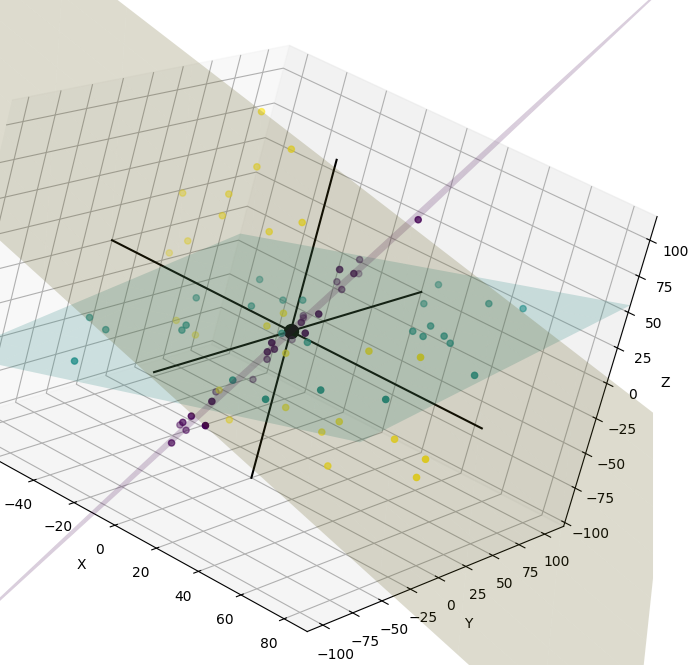
\includegraphics[width=\textwidth]{generated-points.png}
        \end{minipage}
    \end{figure}
    \onslide<4->{
    \textbf{Point Generation} on the plane $(\vec{n},\vec{r}_1,\vec{r}_2)$, parameters $(\maxD,\noise)$:
    \begin{itemize}
        \item random variables $k_1,k_2 \in [-\maxD,\maxD]$ (uniform distribution)
        \item random variable $k_n$ (normal distribution based on $\noise$) 
        \item generate point $p = k_1\vec{r_1} + k_2\vec{r_2} + k_n\vec{n}$ 
    \end{itemize}
    }
\end{frame}


\begin{frame}
    \frametitle{Cost Function (1)}
    % cost function explain what works, wh_at not and why do we need this conditions
    % cost function ~7min with pictures, explain ideas
    % My contribution!!! 
    % Cost function does not depend on the point distribution bounds!!!
    % Steps to assign the cost !!!!!
    % 1. skip triangle where 2 points are close to each other
    % (because may be close to the origin, noise effect, unclear plane spanned by the triangle)
    % 2. skip line like triangles
    % (criteria for almost surely not in the same plane)
    % 3. assign penalty if the noise sum is too large
    \begin{minipage}{0.55\textwidth} 
        \textbf{Triangle} $abc \in \binom{\fSet}{3}$
        \begin{enumerate}
            \onslide<2->{
            \item[(1)] Smallest side $s < \maxD/2$\\
            $\to \cost_{abc} = 0$
            }
            \onslide<3->{
            \item[(2)] Largest angle $\alpha > 150\degree$\\
            $\to \cost_{abc} = 0$
            }
            \onslide<4->{
            \item[(3)] $h_a,h_b,h_c$: distances\\
            to the best fitted plane\\
            containing the origin;\\
            $h_a + h_b + h_c > 3\noise + \tol$\\
            \vspace{5px}
            $\to \cost_{abc} = \frac{(h_a + h_b + h_c) - (3\noise + \tol)}{3\maxD}$
            \vspace{5px}
            }
            \onslide<5->{
            \item[(4)] $h_o$: distance from the origin\\
            to the triangle plane;\\
            $h_o > \frac{10}{\#points}\noise + \tol$\\
            \vspace{5px}
            $\to \cost_{abc} = 0$
            }
        \end{enumerate}
    \end{minipage}
    \begin{minipage}{0.43\textwidth}
        \onslide<2->{
            \begin{tikzpicture}[node distance=30px]
                % nodes
                \node[state, draw=red] (a) {a};
                \node[state, draw=blue] (b) [above right of=a] {b};
                \node[state, draw=blue] (c) [below right of=b] {c};
                \node[state] (o) [above left of=b] {o};
                % edges
                \path[-, ] (a) edge node {} (b);
                \path[-] (b) edge node {} (c);
                \path[-] (c) edge node {} (a);
                \path[-, dashed] (o) edge[red] node {} (a);
                \path[-, dashed] (o) edge[blue] node {} (b);
                
            \end{tikzpicture}
            \hspace{10px}
            \begin{tikzpicture}[node distance=30px]
                % nodes
                \node[state, draw=blue] (a) {a};
                \node[state, draw=blue] (b) [above right of=a, right=10px] {b};
                \node[state, draw=blue] (c) [above right of=a] {c};
                % edges
                \path[-, ] (a) edge node {} (b);
                \path[-] (b) edge node[above] {\small$\noise$} (c);
                \path[-] (c) edge node {} (a);
            \end{tikzpicture}
        }

        \vspace{10px}
        \onslide<3->{
            \begin{tikzpicture}[node distance=30px]
                % nodes
                \node[state, draw=red] (a) {a};
                \node[state, draw=blue] (b) [right of=a, above=7px, right=10px] {b};
                \node[state, draw=blue] (c) [right of=a, right=60px] {c};
                % edges
                \path[-, ] (a) edge node {} (b);
                \path[-] (b) edge node {} (c);
                \path[-] (c) edge node {} (a);
            \end{tikzpicture}
        }

        \vspace{10px}
        \onslide<4->{
            \begin{tikzpicture}[node distance=30px]
                % nodes
                \node[state] (o) {o};
                \node[state, draw=blue] (a1) [right of=o] {a'};
                \node[state, draw=red] (a) [below of=a1, below=10px] {a};
                \node[state, draw=blue] (b1) [right of=o, right=30px] {b'};
                \node[state, draw=blue] (b) [above of=b1, below=3px] {b};
                \node[state, draw=blue] (c1) [right of=o, right=70px] {c'};
                \node[state, draw=blue] (c) [below of=c1, above=10px] {c};
                % edges
                \path[-, dashed] (o) edge[blue] node {} (a1);
                \path[-, dashed] (a1) edge[blue] node {} (b1);
                \path[-, dashed] (b1) edge[blue] node {} (c1);
                \path[-] (a) edge node {} (b);
                \path[-] (b) edge node {} (c);
                \path[-] (c) edge node {} (a);
                \path[-, dotted] (a) edge node[left] {\small $h_a$} (a1);
                \path[-, dotted] (b) edge node[right=6px, below=-6px] {\small $h_b$} (b1);
                \path[-, dotted] (c) edge node[right] {\small $h_c$} (c1);
            \end{tikzpicture}
        }
        
        \vspace{10px}
        \onslide<5->{
            \begin{tikzpicture}[node distance=30px]
                % nodes
                \node[state] (o) {o};
                \node[state, draw=blue] (o1) [below of=o] {o'};
                \node[state, draw=blue] (a) [right of=o1, right=10px] {a};
                \node[state, draw=blue] (b) [right of=o1, right=30px] {b};
                \node[state, draw=blue] (c) [right of=o1, right=60px] {c};
                
                % edges
                \path[-, dashed] (o1) edge[blue] node {} (a);
                \path[-] (a) edge node {} (b);
                \path[-] (b) edge node {} (c);
                \path[-, dotted] (o) edge node[left] {\small $h_o$} (o1);
            \end{tikzpicture}
        }
    \end{minipage}
\end{frame}
    

\begin{frame}
    \frametitle{Cost Function (2)}
        \begin{minipage}{0.55\textwidth}
            \begin{enumerate}
                \item[(5)] for all points $p$:\\
                $h_p$: distance to the best fitted\\
                plane containing the origin;\\
                \vspace{5px}
                \onslide<2->{
                choose $p$ if\\ $h_p < \noise + \tol \land |\vec{p}| > 0.3\maxD$\\
                }
                \vspace{5px}
                \onslide<3->{
                $h_p'$: distance to the best fitted
                plane to all chosen points $p$\\
                containing the origin;\\ 
                }
                \vspace{10px}
                \onslide<4->{
                $\delta_p := \frac{hp' - (\noise + \tol)}{\maxD}$\\
                \vspace{5px}
                $M := \{p \mid p \text{ chosen } \land \delta_p < 0\}$    
                }
                \vspace{10px}
                \onslide<5->{
                $|M| \leq 3 \to \cost_{abc} = 0$\\
                }
                \vspace{10px}
                \onslide<6->{
                $\to \cost_{abc} = 2^{|M|-4} \cdot \sum\limits_{p \in M} \delta_p$    
                }
            \end{enumerate}
        \end{minipage}
        \begin{minipage}{0.43\textwidth}
            \centering
            \begin{tikzpicture}[node distance=30px]
                % nodes
                \node[state] (o) {o};
                \node[state, draw=blue] (a1) [right of=o, right=10px] {a'};
                \node[state, draw=blue] (a) [below of=a1, above=10px] {a};
                \node[state, draw=blue] (b1) [right of=o, right=50px] {b'};
                \node[state, draw=blue] (b) [above of=b1, below=3px] {b};
                \node[state, draw=blue] (c1) [right of=o, right=80px] {c'};
                \node[state, draw=blue] (c) [below of=c1, above=10px] {c};
                \node[state, draw=blue] (p1) [right of=o,left=5px] {p'};
                \node[state] (p) [above of=p1] {p};
                % edges
                \path[-, dashed] (o) edge[blue] node {} (p1);
                \path[-, dashed] (p1) edge[blue] node {} (a1);
                \path[-, dashed] (a1) edge[blue] node {} (b1);
                \path[-, dashed] (b1) edge[blue] node {} (c1);
                \path[-] (a) edge node {} (b);
                \path[-] (b) edge node {} (c);
                \path[-] (c) edge node {} (a);
                \path[-, dotted] (a) edge node {} (a1);
                \path[-, dotted] (b) edge node {} (b1);
                \path[-, dotted] (c) edge node {} (c1);
                \path[-, dotted] (p) edge node[left] {\small $h_p$} (p1);
            \end{tikzpicture}
            \vspace{20px}
            \onslide<3->{
            \begin{tikzpicture}[node distance=30px]
                % nodes
                \node[state] (o) {o};
                \node[state, draw=blue] (p1x) [right of=o,left=5px] {$p_1'$};
                \node[state, draw=blue] (p1) [above of=p1x] {$p_1$};
                \node[state, draw=blue] (p2x) [right of=o, right=10px] {$p_2'$};
                \node[state] (p2) [above of=p2x, above=5px] {$p_2$};
                \node[state, draw=blue] (p3x) [right of=o, right=30px] {$p_3'$};
                \node[state, draw=blue] (p3) [below of=p3x, above=10px] {$p_3$};
                \node[state, draw=blue] (p4x) [right of=o, right=60px] {$p_4'$};
                \node[state, draw=blue] (p4) [above of=p4x, below=5px] {$p_4$};
                \node[state, draw=blue] (p5x) [right of=o, right=80px] {$p_5'$};
                \node[state, draw=blue] (p5) [below of=p5x] {$p_5$};
                % edges
                \path[-, dashed] (o) edge[blue] node {} (p1x);
                \path[-, dotted] (p1) edge node[left] {\small $h_{p_1}'$} (p1x);
                \path[-, dashed] (p1x) edge[blue] node {} (p2x);
                \path[-, dotted] (p2) edge node[left] {\small $h_{p_2}'$} (p2x);
                \path[-, dashed] (p2x) edge[blue] node {} (p3x);
                \path[-, dotted] (p3) edge node[right=1px] {\small $h_{p_3}'$} (p3x);
                \path[-, dashed] (p3x) edge[blue] node {} (p4x);
                \path[-, dotted] (p4) edge node[left] {\small $h_{p_4}'$} (p4x);
                \path[-, dashed] (p4x) edge[blue] node {} (p5x);
                \path[-, dotted] (p5) edge node[left] {\small $h_{p_5}'$} (p5x);
            \end{tikzpicture}
            }
        \end{minipage}
\end{frame}
\section{Experiments and Evaluation}
\frame{\tableofcontents[currentsection]}


\begin{frame}
    \frametitle{Experiments}
    My laptop characteristics, 
    Random cubic subspace instances with different seeds 
    max point component size 100 (noise are the percents then)
    no noise 0,
    small noise 1,
    significant noise 3,
    large noise 5,
    (Table: instance size + noise + instance count)
\end{frame}


\begin{frame}
    \frametitle{Cost Function Evaluation}
    blue and red dots,
    conflicts and and their effect
    (picture of the typical cost function evaluation)
\end{frame}

\begin{frame}
    \frametitle{Experiment Results for 3x7 Points}
    3x7 points: all results +
    time-optimality-accuracy (min-max-average) 
\end{frame}

\begin{frame}
    \frametitle{Experiment Results}
    3x(7x12x17x22) time-optimality-accuracy (min-max-average) 
    DIAGRAM!!! 
    mention the coefficients to prove the efficiency, partial optimality and accuracy!!!
\end{frame}



\section{Conclusion}
\frame{\tableofcontents[currentsection]}


\begin{frame}
    \frametitle{Conclusion}
    % C++, features list
    % cost function determined experimentally
    % high accuracy and efficiency shown in the experiments
    % future work: 
    % optimize to improve the time complexity and get better scalability
    % parallelize the condition checks as an option
    % improve the cost function to overcome the partial optimality loss
    % using the better parameters and more advanced criteria
    \vspace{-5px}
    \onslide<1->{
    \begin{enumerate}
        \item Implementation of the partial optimality algorithm:
        \begin{itemize}
            \item arbitrary sample type
            \item sparse cost representation
            \item pair labeling and triple cuts
            \item reasonable adjustments of the partial optimality conditions
            \item self-explaining logs
        \end{itemize}
        \onslide<2->{
        \item Subspace instance generation using linear algebra methods,\\
        geometric cost function $\cost$:
        \begin{itemize}
            \item high accuracy (over 75\%)
            \item significant noise tolerance ($\noise \geq 1$)
            \item $O(k \cdot n^6)$ for $n=\text{\#points}$ and a small $k$
        \end{itemize}
        }
    \end{enumerate}
    }
    \vspace{5px}
    \onslide<3->{
    \textbf{Future Work}:
    \begin{itemize}
        \item optimize and parallelize the algorithm
        \item overcome the partial optimality loss for $\cost$
        \item determine better parameters for $\cost$
        \item update $\cost$ with advanced criteria
    \end{itemize}
    }
\end{frame}


\begin{frame}
    \frametitle{References}
    \textbf{My program, scripts and presentation:}
    \url{https://github.com/Vovsanka/ResearchProjectML}\\
    \vspace{20px}
    \textbf{Bibliography:}\\
    \vspace{5px}
    \printbibliography
\end{frame}



\end{document}